\documentclass[12pt,a4paper]{report}
\usepackage[T1]{fontenc}
\usepackage[utf8]{inputenc}
\usepackage[english]{babel}
\usepackage{hyperref}
\usepackage{graphicx}
\usepackage{caption}
\usepackage{amsmath}
\captionsetup{figureposition=bottom, font=small}


\title{Deblurring Images with Autoencoders Neural Networks}
\author{Francesco Bonzi and Andrea Zanellati}
\date{}

\begin{document}
\maketitle
\newpage
\tableofcontents
\newpage

\section*{Introduction}
\addcontentsline{toc}{section}{Introduction}
Blurring is the process of altering a region of a signal generally due to  a weighted sums of neighboring regions of the same signal. In the case of image blurring, a pixel’s value is affected by the adjacent pixels. There are several causes for blurring artefacts such as\cite {P&V&G}: 
\begin{itemize}
\item \textit{motion blur} due to movement of the object or imaging system;
\item \textit{out of focus} due to incorrect focus such as long exposure time;
\item \textit{Gaussian blur}, that is the result of blurring an image by a Gaussian function, with the main purpose to reduce the details of an image.
\end{itemize}

Deblurring is the process of removing blurring artifacts from images, that is to say that given a blurred image $B$ we try to recover the sharp image $S$. The problem can be mathematically represented with the equation \begin{equation} B = S * K \end{equation} where $K$ represents the unknown linear shift-invariant Point Spread Function (PSF). This function describes the response of an imaging system to a bright pixel (point source) by expressing the degree to wich an optical sistem blurs a point of light.

PSF play a key role in standar deblurring techniques and we can distingush two different families: on one hand \textit{blind deconvolution methods} focus on recovering the unknown PSF, on the other hand \textit{non-blind methods} rely on a known PSF for performing robust deconvolution. Deblurring techniques can be split into two distinct problems: recovering the PSF by solving an inverse ill-posed problem and recovering the initial estimate using a known PSF. There are several numerical techniques developed to address the problem \cite{H&Al}. In our project we deal with a deep neural network approach which can be collocated among the blind deblurring techniques where the PSF function is represented by mean of the neural network. The input of the training system is a set of blurred images and the target output is the corresponding sharp images. In a way, the training phase of the neural network can be seen as the  PSF recovering while the prediction phase is the second part of the deblurring problem. In particular we have developed three \textit{autoencoder} architectures, whose main features are highlighted in the following section. 

Two different Dataset are considered: CIFAR10 and REDs. As regards the first one, it is a set of 60000 low resolution colour images with dimension 32x32. We randomly applied a Gaussian Blur Filter to create a dataset with a sharped and a blurred version of each image. As concerns REDs, it is a dataset for video-deblurring and super-resolution but we consider it as a set of high-resolution colour images with motion blur due to moving objects or camera movements. The top quality images are organized in 270 videos consisting in 100 frames each with size 1280x720 and it was not possible for us to handle the training phase with this dataset with the available computational resources. To overcome the problem, we decided to work with the low resolution version of the same dataset which has 320x180 size images, on which a division into patches was applied in order to reduce the number of needed neurons in the network. In section 4 we will discuss in details this strategy.

The project focuses on comparing the different autoencoders according to three main criteria:
\begin{enumerate}
\item Using different structures which are similar for the number of parameters that must be fit during the training;
\item Using different number of layers and filters in the setting of each kind of autoencoder;
\item Using different loss functions.
\end{enumerate}

The experiment with CIFAR10 was conducted considering all the three criteria mentioned above. For REDs, given the high computational cost, we limited our investigation to a comparison on the three different structures of autoencoders.

In the next section we describe the architectures of the designed autoencoders. Section 2 is dedicated to the introduction of some loss functions and accuracy metrics and how they have been used to train and assess our models. Section 3 and 4 present the results obtained on the two Datasets mentioned above. In particular section 4 is dedicated to REDs and we will also discuss the implemented strategy to locally deblur images. In the $5^{th}$ section we discuss other strategies that we have hypothesized to address the deblurring problem: the first is a multi-classifier network for \textit{motion field estimation}; the second is inspired by a research article\cite{G&E&B} on \textit{style transfer}. Finally, last section is the conclusion of this report in which we sum up the main results of the project.
 
\section{Architectures of the Neural Networks}
An autoencoder is an artificial neural network that learns to copy its input to its output. It is constituted by two main parts: an encoder that compress the input into a lower-dimensional code, and a decoder that maps the code to a reconstruction of the original input. The code is a compact “summary” or “compression” of the input, also called the latent-space representation. In our autoencoder architectures the main goal is not to generate an exact copy of the original input, but rather to achieve a good representation by changing the reconstruction criterion. Indeed, the networks take a partially corrupted input and are trained to recover the original undistorted input. In practice, the objective of deblurring autoencoders is that of cleaning the corrupted input, or deblurring. In order to address the encoding problem Convolutional Neural Network layers (CNN) are employed, while the decoding phase is faced with deconvolution layers. CNN layers with different filters have the power to extract patterns and the main features from the input images which are saved in the latent space representation. Three different architectures have been developed based on autoencoder structure and for each of them we designed different version. In figure \ref{table_params} there is a comparison between the number of total parameters to train in each network.

\begin{figure}[hbtp]
\centering
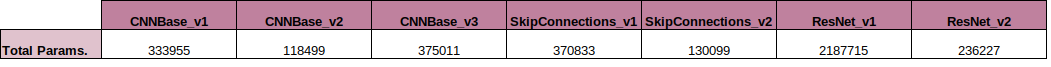
\includegraphics[scale=0.55]{params_table.png}
\caption{Table of the toltal number of parameters in each network}\label{table_params}
\end{figure}

\subsection{Plain Network}
Our simplest architecture is a plain symmetric network (hereinafter referred to as "CNN Base") with three convolutional layers (encoders) and three deconvolutional layers (decoder) followed by a fourth deconvolution layer which returns the output image with the number of channels equal to those of the input image. ReLU is used as activation function as suggested in the literature when using CNN to avoid gradient vanishing descent problem. We designed two different schemes. 

The first version can be represented with the following structure: 
\begin{equation}
C_{32}^{3,1} - C_{64}^{3,1} - C_{128}^{3,1} - D_{128}^{3,1} - D_{64}^{3,1} - D_{32}^{3,1} - D_{3,p}^{3,1} 
\label{CNNbase_v1}
\end{equation}

where $C_n^{k,s}$ indicates a convolutional layer, $n$ is the number of filters which are applied with kernel size $k$ and stride $s$. $D_n^{k,s}$ is a deconvolutional layer where $n, k, s$ have the meaning already stated. In the last layer a $p$ is added next to the number of filters to mean that the deconvolution is applied with a padding that ensures that the output image dimension changes only as regards the number of channels.

The second version has always a plain symmetric structure but it has been designed deeper but with less filters per layer. By using the same notation introduced above we have: 

\begin{equation}
5C_{8}^{3,1} - 5C_{16}^{3,1} - 5C_{32}^{3,1} - 5D_{32}^{3,1} - 5D_{16}^{3,1} - 5D_{8}^{3,1} - D_{3,p}^{3,1} 
\label{CNNbase_v2}
\end{equation}

where the number before each letter indicates the number of layers with the given features. 

The second version has about half parameters compared to the first one, therefore we have decided to design a third version deeper than the first one but with a similar number of parameters. It can be represented by the scheme:

\begin{equation}
4C_{16}^{3,1} - 4C_{32}^{3,1} - 4C_{64}^{3,1} - 4D_{64}^{3,1} - 4D_{32}^{3,1} - 4D_{16}^{3,1} - D_{3,p}^{3,1} 
\label{CNNbase_v2}
\end{equation}

\subsection{Skip Connections}

Following the proposal in \cite{M&Al} we have modified the plain network schemes described in \eqref{CNNbase_v1} and \eqref{CNNbase_v2} by adding \textit{symmetric skip connections}. The main purpose is to pass information of the convolutional feature maps to the corresponding deconvolutional layers. This operation totally changes how the network works; instead of directly learning the mappings from the input $X$ to the output $Y$, we consider that the network estimates a residual of corruption $\emph{F}(X)$ which can be added to the input $X$ allowing to reconstruct the uncorrupted image. In other terms, we have that $Y = X + \emph{F}(X)$.

As regards the scheme of the proposed networks, they can be represented as follow:

\begin{equation}
C1_{32}^{3,1} - C2_{64}^{3,1} - C3_{64}^{3,1} - C4_{128}^{3,1} - D5_{128}^{3,1} - D6_{64}^{3,1} - S7_{C2} - D8_{32}^{3,1} - S9_X - D10_{3,p}^{3,1} 
\end{equation}

\begin{equation}
5C_{8}^{3,1} - 10C_{16}^{3,1} - 5C_{32}^{3,1} - 5D_{32}^{3,1} - 5D_{16}^{3,1} - S_{C6} - 2D_{8}^{3,1} - S_{C4} - 2D_{8}^{3,1} - S_{C2} -D_{8}^{3,1} - S8_X - D_{3,p}^{3,1} 
\end{equation}

where the notation previously introduced is still valid and it has been expanded with the number next to each capital letter which indicates the layer number in the network. $S_{L}$ is the symbolic representation of an element-wise sum between the output of the previous layer and those of layer $L$. The $X$ is used to denote the input image. 

The main expected advantage in the use of skip connections concerns the optimization process during the backpropagation while training the network. Optimizing for the corruption is expected to converge better than optimizing for the clean image. In the extreme case, if the input is a clean image, it
would be easier to push the network to be zero mapping, which represents the absence of corruption, instead of fitting an identity mapping which leaves unchanged the image with a stack of nonlinear layers.

\subsection{Residual Network}
The last autoencoder structure is inpired by ResNet \cite{N&Al}\cite{H&X&R} and it includes some residual blocks. The main idea under this architectures is similar to the one used in the previous one: we are adding some \textit{shortcuts} which are useful to estimate the residual. Differently from the skip connections approach, a residual block in this architecture passes the information of the convolutional feature maps two layer ahead, while previously we designed the network in a symmetric way where skip connections where a bridge between correspondent convolutional and deconvolutional layers. In a sense, the network is a Long Short-Term Memory approach without gates. 

\begin{figure}[hbtp]
\centering
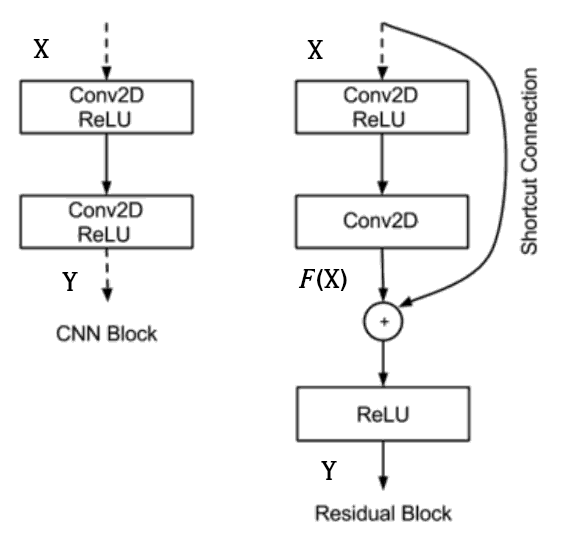
\includegraphics[scale=0.5]{ResidualBlock.png}
\caption{Comparison between a Plain CNN Network and a Residual Block}\label{ResNet}
\end{figure}

As shown in Figure \ref{ResNet}, a residual block consists of two convolutional layers, the first of which uses ReLU as an activation function. Said $X$ the input of the residual block and $\emph{F}(X)$ the output of the second convolutional layer, the global output of the Residual Block is expressed by a ReLU evaluation of $X +\emph{F}(X) $, and therefore $\emph{F}(X)$ can be interpreted as a term of approximation of the corruption applied to the input image.

We developed two schemes for Residual Networks, the one represented in (\ref{ResNet_v1}) is shallower but with an higher number of filters applied in each layer than the second version in (\ref{ResNet_v2}).
\begin{equation}
C_{32}^{5,2} - R_{32}^5 - C_{64}^{5,2} - R_{64}^5 - C_{128}^{3,2} - R_{128}^3 - D_{128}^{3,2} - R_{128}^5 - D_{64}^{5,2} - R_{64}^5 - D_{32}^{8,2} - D_{3,p}^{3,1} 
\label{ResNet_v1}
\end{equation}

\begin{equation}
C_{8}^{5,2} - 2R_{8}^5 - C_{16}^{5,2} - 2R_{16}^5 - C_{32}^{3,1} - 2R_{32}^3 - D_{32}^{3,1} - 2R_{32}^5 - D_{16}^{3,1} - 2R_{16}^5 - D_{8}^{8,1} - D_{3,p}^{3,1} 
\label{ResNet_v2}
\end{equation}

The two schemes can be interpreted with the already introduced notation with the extension of $R_n^k$ which indicates a residual block where each convolutional layer uses $n$ filters of size $k$.

\section{Loss Functions}
The loss function used during the training of a neural network plays a crucial role to determine the quality of the output. As suggested in \cite{Z&G&F}, the \textit{Mean Square Error} (MSE) is not the best metric to use to define the loss function for images restoration problem. Some perceptually motivated metrics have been introduced in the literature and seem to outperform the results obtained using standard metrics. Therefore, we have defined a loss function based on \textit{Structural Similarity Index Measure} (SSIM) and we have compared the output quality. In order to compare the results we also used other two metrics of evaluation: the \textit{Mean Absolute Error} (MAE) and the \textit{Peak Signal-to-Noise Ratio} (PSNR). In this section we briefly recall the definitions of these metrics and their meanings. 

\subsection{Perceptually motivated metrics}
SSIM is a perception-based model that estimates image degradation as a combination of structural information which includes luminance, contrast and stucture terms. In a sense, it gives an estimation of perceived change considering those aspects which are relevant to human eyes. Talking of structural information means considering that the pixels have strong inter-dependencies especially when they are spatially close. 

If we consider two correspondent windows $x$ and $y$ in the comparing images (generally sharped and predicted images), their SSIM index is defined as a weighted combination of luminance $l(x,y)$, contrast $c(x,y)$ and stucture terms $s(x,y)$ expressed in terms of average, variance and covariance of $x$ and $y$. When the combination is expressed as a simple product of the three terms, it turns in the following formula:

\begin{equation}
SSIM_{local}(x,y) = \frac{(2\mu_x\mu_y+c_1)(2\sigma_{xy}+c_2)}{(\mu_x^2+\mu_y^2+c_1)(\sigma_x^2+\sigma_y^2+c_2)}
\end{equation}

where $\mu_x$ and $\mu_y$ are rispectivly the average pixel value of the two windows $x$ and $y$, and $\sigma_x$, $\sigma_y$ and $\sigma_{xy}$ are their variance and covariance. The constant terms $c_1$ and $c_2$ are used to stabilize the division with weak denominator and they have default values. In our project the \textit{global SIMM index} is computed with the tensorflow function tf.image.ssim. Accordingly to the description in \cite{W&B}, a local SIMM value is computed for each correspondent 11x11 windows by using a Gaussian filter with standard deviation of $1.5$ samples and the global SIMM index for the images is obtained as their mean value. Denoting with $X$ and $Y$ the comparing images, with $M$ the total number of windows and using the subscript $i$ to enumarate them, we have:

\begin{equation}
SSIM = \frac{1}{M}\sum_{i=1}^M SSIM_{local}(x_i,y_i)
\end{equation}

In general, SSIM is defined for grayscale images and assumes a value in $[-1,1)$ where an high value indicates that there is a great similarity between the two images. The function \emph{tf.image.ssim} of Tensorflow recives in input two image batches to compare and returns a tensors with the SSIM index computed for each couple of correspondent images. When a color image is given as input the SSIM index is evaluated on each channel and we have assumed their mean value as gloabal SSIM index.

Moreover, a Structural Dissimilarity Index Measure (DSSIM) can be derived from SSIM as follow:

\begin{equation}
DSSIM(X,Y) = \frac{1-SSIM(X,Y)}{2}
\end{equation} 

which assumes values in the range $(0,1]$ and that can be used to define a loss function to minimize in a restoration images problem. Our loss function based on SSIM, named SSIMLoss, is defined as $SSIMLoss = 2 DSSIM$.



\subsection{Other Metrics and their use}
As stated before, we have used a SSIM based function as main loss function and, for CIFAR10 dataset we have also tried the training of the networks by using MSE as loss function. MAE and PSNR, instead, are only used as accuracy metrics to evaluate the output quality. In \cite{Z&G&F} MAE is suggested as loss function with better results than MSE when images have big plain area, where problems are mostly related to changes in colours and lights than those affecting shapes and figures. We didn't recognize this kind of features as characterizing the given datasets, so we prefered to use MSE as standard loss function to compare with the stuctural dissimilarity index. There are two main uses of all these metrics.

Firstly, they can be used to compare the different architectures. On one hand, we can have an estimation about the quality of the restored images both on training and test dataset; on the other hand, we can highligth overfitting behaviour by comparing the metric values for training and validation sets. In particular, we can detect overfitting if the accuracy values on training data decrease while those related to the validation data are increasing.


Secondly, the loss function updating in different epochs is used to determine an \textit{early stop criterion}. More precisely, if the value of the loss function does not have a significant improvement for a predetermined number of epochs, the training is stopped. In our experiments we used a tolerance for improvement equal to $10 ^ {- 4}$ setting a parameter of "patience" of $3$ epochs.

To conclude this section, we recall the definitions of the metrics used in this project. In the following formulas, we refer to a sharped grayscale image with $X$, to the correspondent predicted image with $Y$ and we use $p$ to denote the position of a generic pixel and $n$ as the total number of pixels per image. The definitions are given as follow:
 
\begin{equation}
MSE(X,Y) = \frac{1}{n}\sum_{p\in X,Y} (X(p)-Y(p))^2
\end{equation}

\begin{equation}
MAE(X,Y) = \frac{1}{n}\sum_{p\in X,Y} |X(p)-Y(p)|
\end{equation}

\begin{equation}
PSNR(X,Y) = 20 \log_{10} \left( \frac{MAX_I}{\sqrt{MAE(X,Y)}}\right) 
\end{equation}

In the PSNR definition the term $MAX_I$ represents the maximum value for a pixel of an image. All the previous formula can be extended for color images considering the mean of the value computed on each channel.

\section{First Experiment: CIFAR10}
In this section we are going to sum up the main results obtained by using the neural networks already described with CIFAR10 dataset.

\begin{figure}[hptb]
\centering
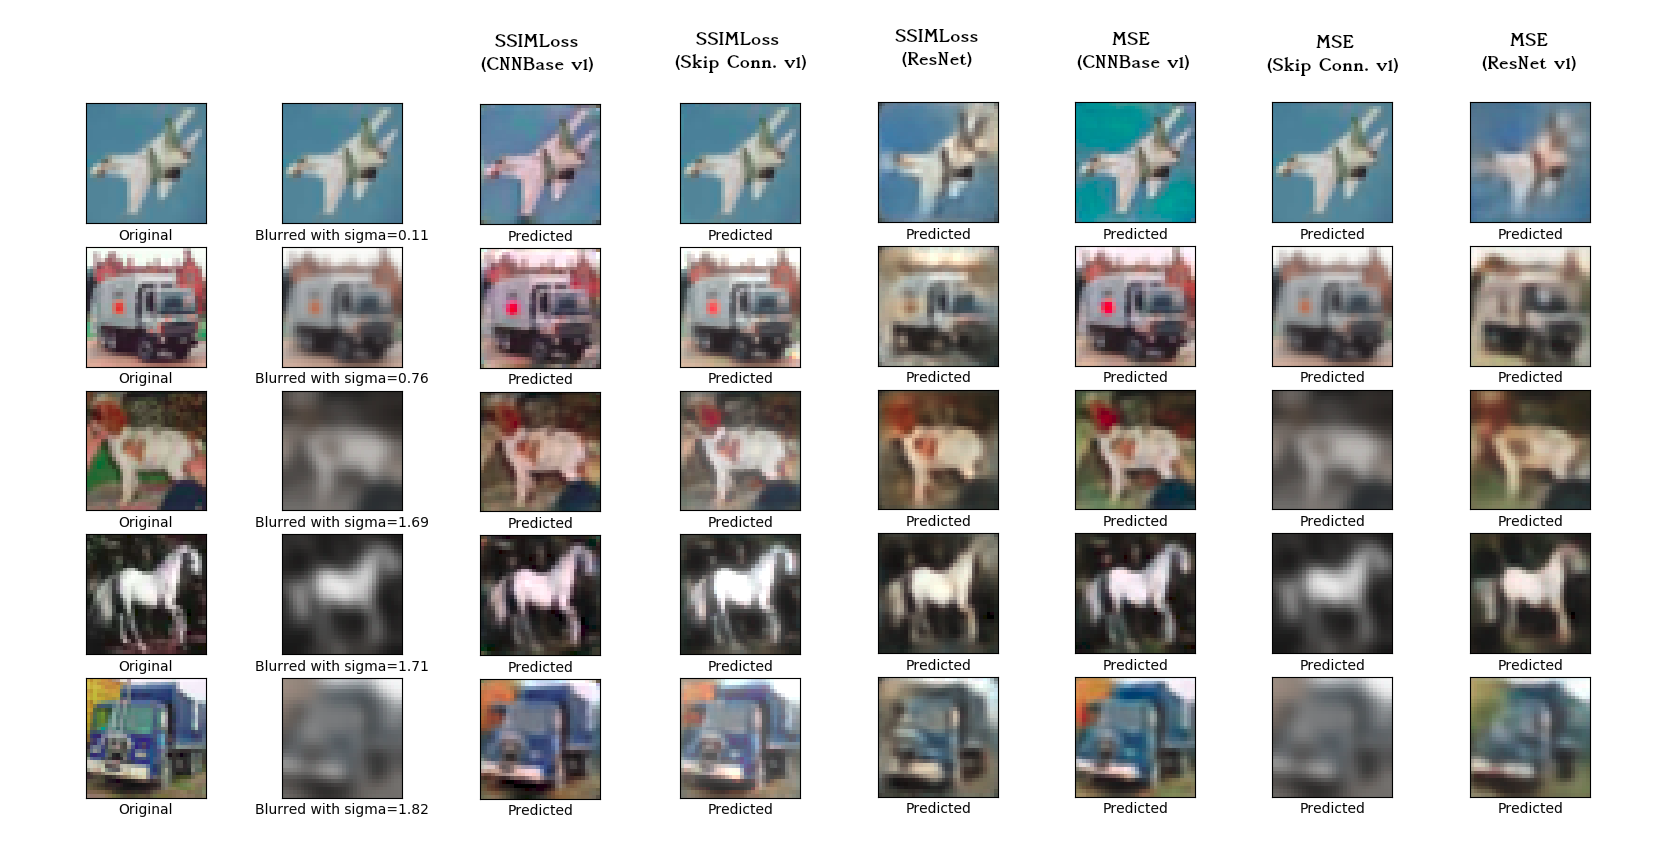
\includegraphics[scale=0.26]{Outputs_comparison.png}
\caption{Output examples}
\label{CIFAR10Output}
\end{figure}

In Figure \ref{CIFAR10Output} we have some output examples obtained by using the different models. We have decided to report the best of the results between the two implemented versions for each kind of architecture (CNN base, Skip Connections and ResNet).
Generally speaking, we can observe that the basic CNN architecture works better than the other, even if the recnostructed colors in the Skip Connections network outputs are more similar to those in the original pictures. The worst results are those obtained with the ResNet architecture. In particular, the network is able to recover a global shape of the main object in the image, but a lot of information about colors and details remains undetected.

\begin{figure}[hptb]
\centering
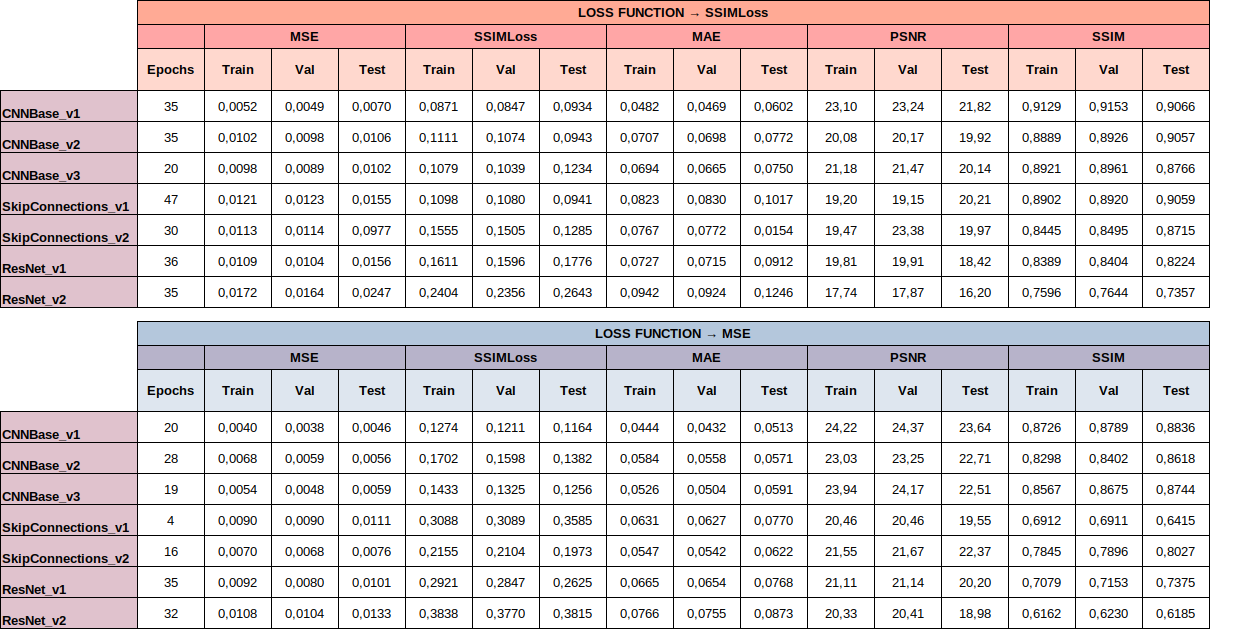
\includegraphics[scale=0.45]{table.png}
\caption{Accuracy Indexes Table on CIFAR10}
\label{Table1}
\end{figure}

We can better evaluate the quality of the outputs by considering some metrics as discussed in the previous section. The tables in Figure \ref{Table1} sum up the values registered for the different architectures by using as loss function both SSIMLoss and MSE. We can highligts three main points:

\begin{figure}[hptb]
\centering
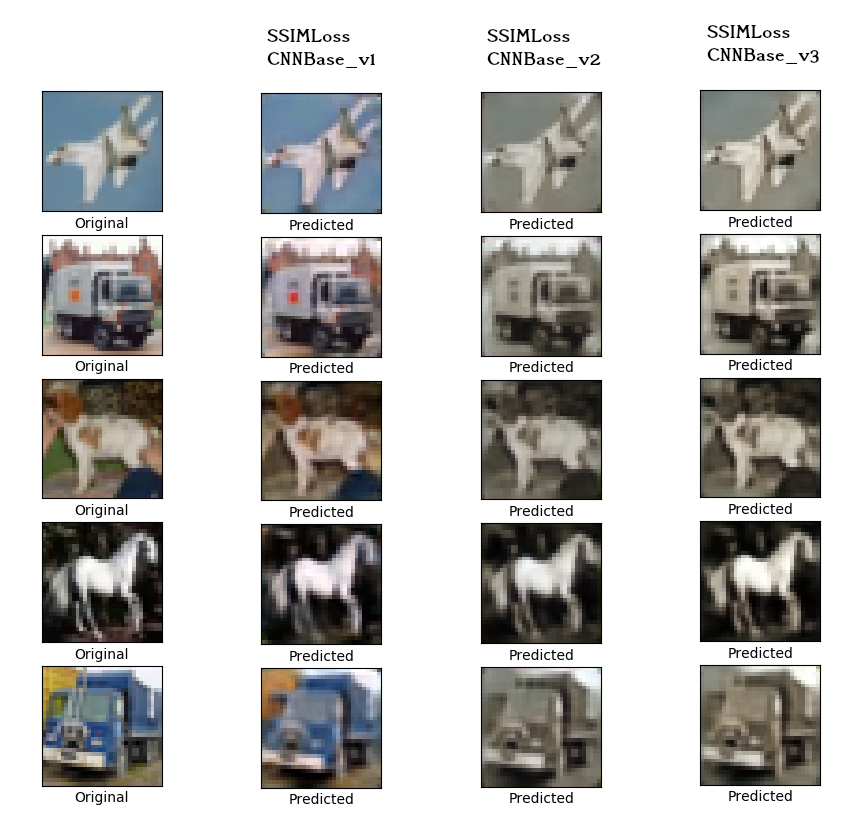
\includegraphics[scale=0.45]{CNNBase_comparison.png}
\caption{Outputs comparison with different version of CNNBase scheme}
\label{CNNBase_comparison}
\end{figure}

\begin{itemize}
\item The number of epochs for corresponding networks with different loss functions is always smaller in the case of training with optimization of the MSE. This means that in those cases the stop criterion is reached earlier with respect to the training with SIMMloss.
\item For each structure the shallower network with a larger number of nodes performs better than the deeper network of the same kind. We suppose that this may be a consequence of the number of filters used which favors the coding of characterizing patterns. In particular, we can observe in figure \ref{CNNBase_comparison} that version 2 and 3 of CNNBase, which has the best performance in its first version, almost completely lose the color information showing restored images in the chromatic scale of gray.
\item Comparing different structures trained with the same loss function we see that the best results are performed by the basic CNN scheme network, and this confirms the observation made by comparing the outputs in Figure \ref{CIFAR10Output}. In particular, SSIM attests a very good performance for the CNNbase network when trained with SSIMLoss as loss function; in fact, the value of the index is higher than $0.9$ even for the images used as test.
\end{itemize}


\begin{figure}[hptb]
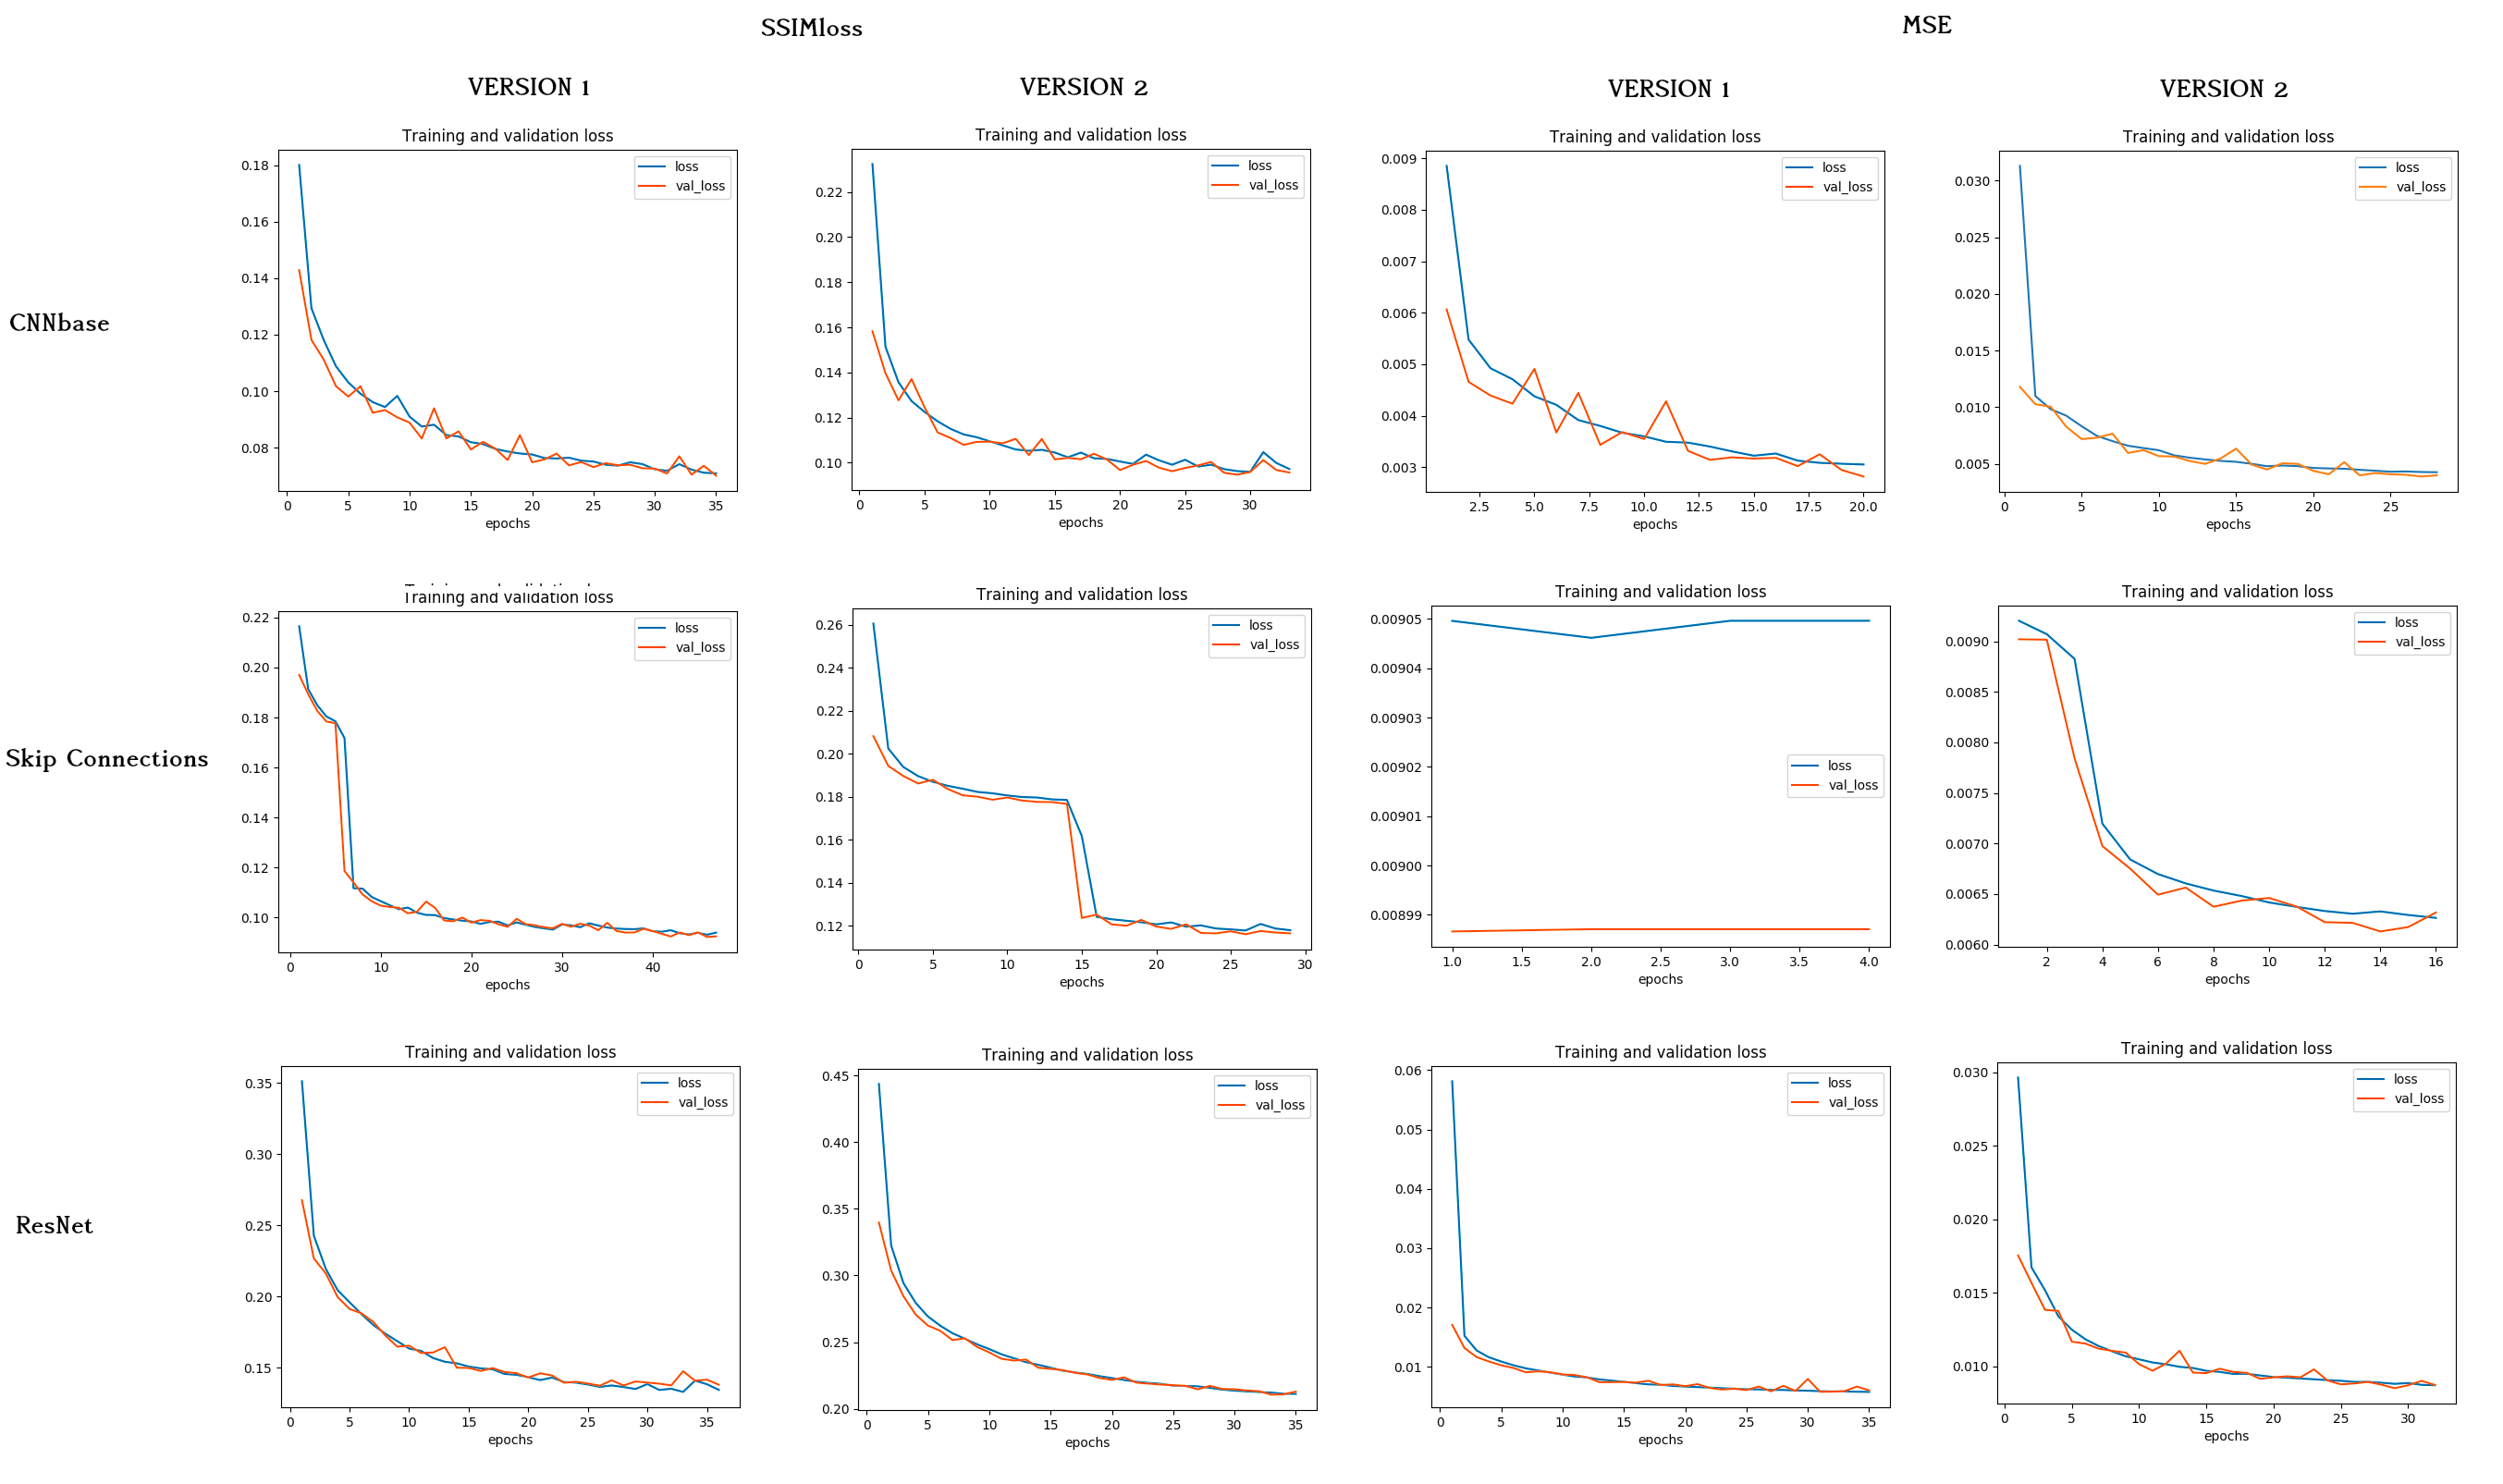
\includegraphics[scale=0.21]{Loss_accuracy_comparison.png}
\caption{Loss Accuracy Comparison between different networks on CIFAR10}
\label{CIFAR10Loss}
\end{figure}

In Figure \ref{CIFAR10Loss} we have collected the loss function behaviours for each network during the training phase. The graphs suggest further confirmation of the points highlighted above and we can recognize a fast decrease of the loss function in the early epochs, followed by a slower decrease. The trend on the training set is characterized by a regular decrease while small fluctuations can be noticed on the validation set. Moreover, the loss function curves for the validation set have the same decreasing behaviour of the correspondent curves on the trainig set. This is a good feature because it means the network is not overfitted; furthermore, the fact that the values for all the considered metrics are similar for training, validation and test datasets is a confirmation of no - overfitting.


\section{Second Experiment: REDs}
The deblurring problem on the REDs dataset is significantly more challenging compared to the one on CIFAR10, due to the images resolution and the size of the dataset. To tackle the computational cost problem we intervened in two ways. As for the technical aspects, we decided to look for a more performing machine using a virtual machine on Azure \footnote{The VM has the following features: E4 Standard v3 (4 virtual CPUs, 32 GB memory) Linux 18.04-LTS operating system}. Regarding the modelization approach, in order to handle the problem we have decided to work locally on each image by splitting it into patches.

The code provides for the possibility of establishing the size of the patches in each image, and consequently their number. In our experiment we use 4x2 patches when we train or predict with CNN Base or Skip Connections and we have 3x2 patches for ResNet architectures. We designed the division into patches to be partially overlapping, with a number of overlapping pixels equal to twice the number of convolutions in the network. This means that the pixels that are left out during the training of the network due to the stride effect (fixed equal to 1) do not affect the output of the central pixels of each patch that will then be used in the restored image.

\begin{figure}[hptb]
\centering
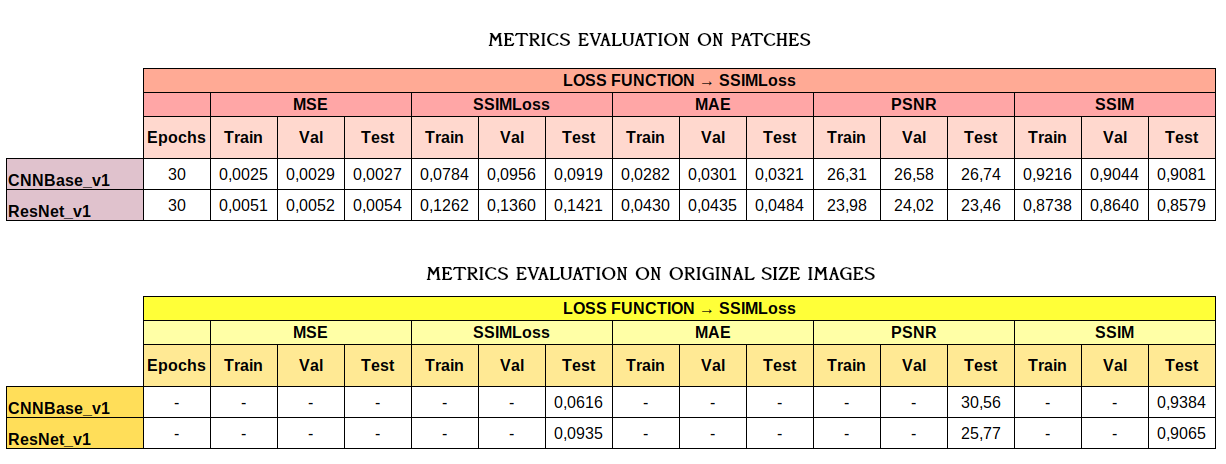
\includegraphics[scale=0.45]{REDs_table.png} 
\caption{Accuracy Indexes Table on REDs patches}
\label{REDs_table}
\end{figure}

Unlike what we did in the experiment on CIFAR10, we limited ourselves to training networks in version 1, i.e. with fewer layers and more filters, and always using SSIMLoss as a loss function. This is mainly due to the high computational cost of training with REDs dataset and so we decided to explore the outputs of those networks that produce better results on CIFAR10. Also in this case the best results are obtained from the CNN Base network with a PSNR index of $26.31$ on the train dataset and SSIM of approximately $0.92$ as we can see in figure \ref{REDs_table}(a) which reports the metrics related to network outputs on patches. We have also tested the network SkipConnections but the training stop after 4 epochs due to the early stop criterion without any learning.

\begin{figure}[hptb]
\centering
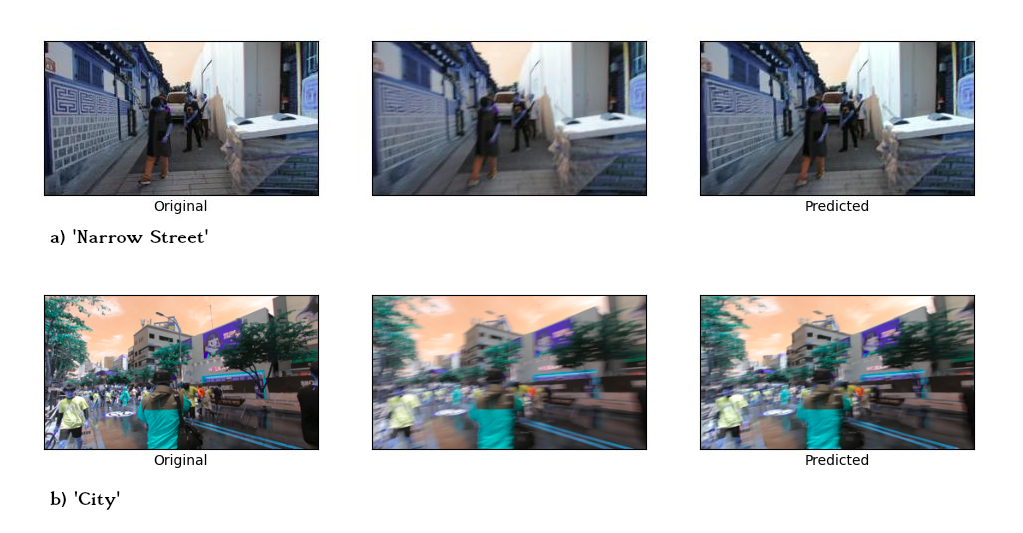
\includegraphics[scale=0.48]{REDs_CNNBase_Outputs.png} 
\caption{CNNBase Outputs on REDs Dataset}
\label{REDs_outputs_CNNBase}
\end{figure}

In order to evaluate the effectiveness of the networks on the global deblurring problem we decided to calculate the SSIM and PSNR indices on some test images reconstructed in their globality. The results are really satisfying with a particular appreciation for the CNN Base network where SSIM has a value of $0.93$ and PSNR is equal to $30.56$. These values were computed on 50 random frames per 30 videos in the test dataset. An unexpected result is the fact that the metrics are better on  restored images in their entirety rather than on individual patches. We have interpreted this result as a consequence of the overlapping factor used in images rebuilding. Except for the contour pixels in the images at original size, in the central part deblurring is conducted so that there are no undesirable effects due to padding or to the reduction of the number of pixels.


In figure \ref{REDs_outputs_CNNBase} we have two examples of outputs on test images with the CNNBase network. The quality already assesed by the metrics is also appreciable in a qualitative observation of the outputs. 

In figure \ref{REDs_outputs_CNNBase_Zoom} the pictures show some zoom details of the images where we notice a very good restoration work by the network.

\begin{figure}[hptb]
\centering
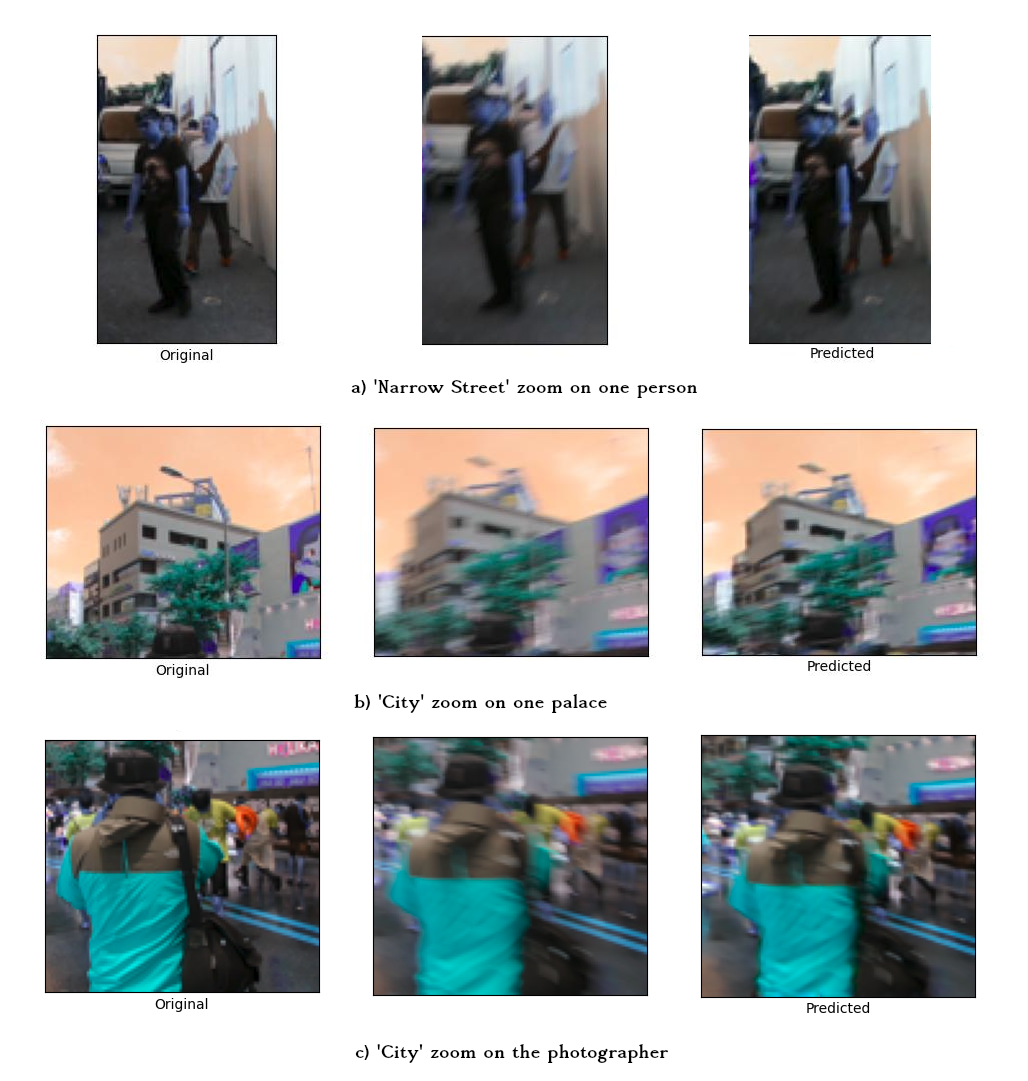
\includegraphics[scale=0.35]{REDs_CNNBase_Outputs_Zoom.png} 
\caption{CNNBase Zoomed Outputs on REDs Dataset}
\label{REDs_outputs_CNNBase_Zoom}
\end{figure}

 
By comparing these results with those obtained with ResNet network (figures \ref{REDs_ResNet_Outputs} and \ref{REDs_ResNet_Outputs_Zoom}) it is evident that they have a lower quality. However, some information of the sharped images are recovered also in this case, such as the palace shape. In general, both the networks perform better in in restoring parts of images with well-marked outlines. For example, in the "City" image, the part relating to the trees maintains a higher blur than the details shown in the figure \ref{REDs_outputs_CNNBase_Zoom} and \ref{REDs_ResNet_Outputs_Zoom}.


\begin{figure}[hptb]
\centering
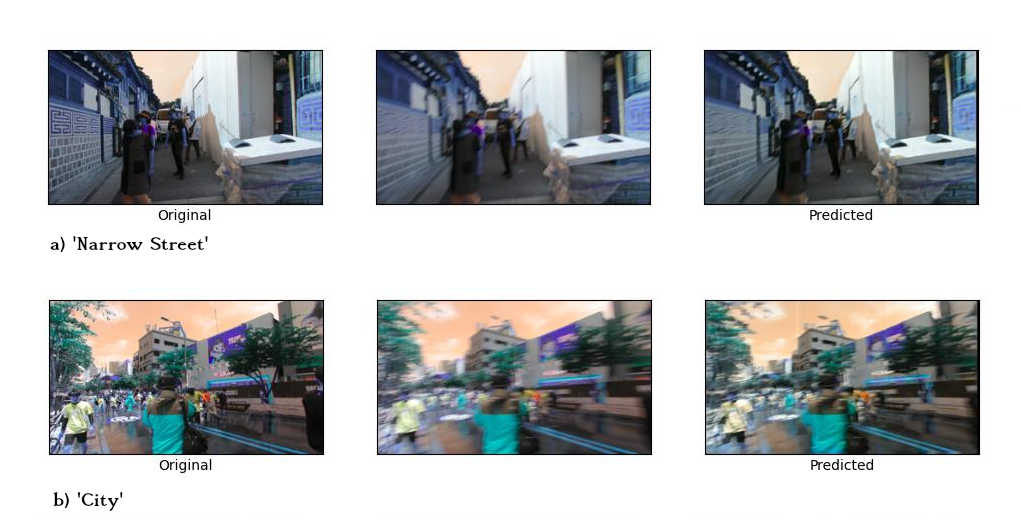
\includegraphics[scale=0.5]{REDs_ResNet_Outputs.png} 
\caption{ResNet Outputs on REDs Dataset}
\label{REDs_ResNet_Outputs}
\end{figure}

\begin{figure}[hptb]
\centering
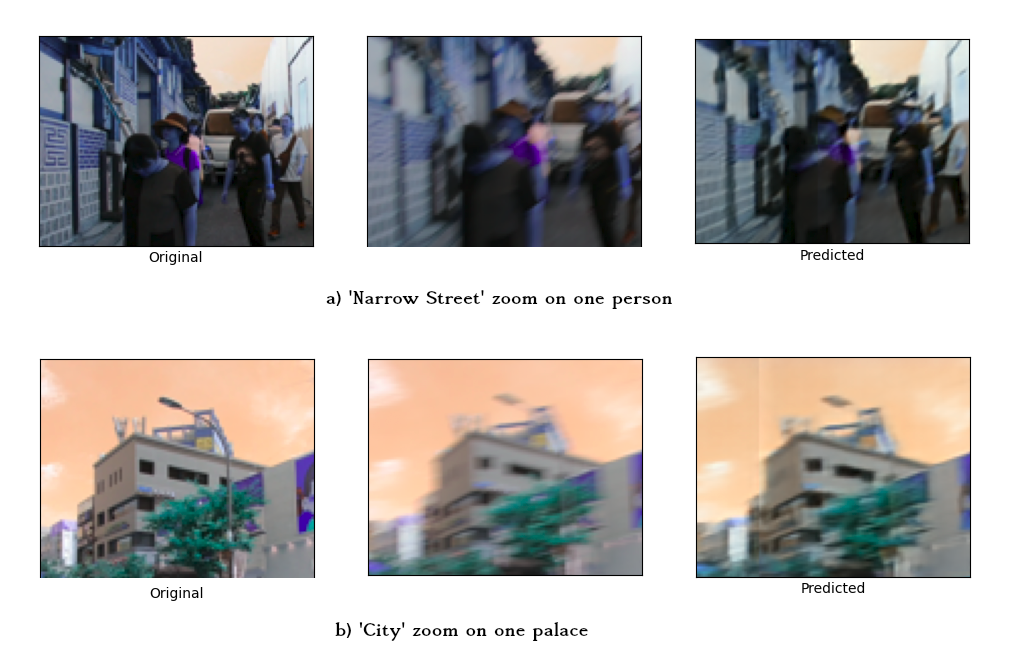
\includegraphics[scale=0.35]{REDs_ResNet_Outputs_Zoom.png} 
\caption{ResNet Zoomed Outputs on REDs Dataset}
\label{REDs_ResNet_Outputs_Zoom}
\end{figure}

We can show also the loss function behavior during the epochs evolution (figure \ref{Loss_accuracy_comparison_REDs}). The decrease considerations made for the CIFAR10 dataset also apply, even if in this case the training stop occurred before the intervention of the early stop criterion and therefore the platau area is not included in the graph. Better results could be obtained by setting an epoch limit higher than 30, but considering the already satisfactory outputs and the computational and time costs of a new training set on a greater number of epochs, this path has not been developed.

\begin{figure}[hptb]
\centering
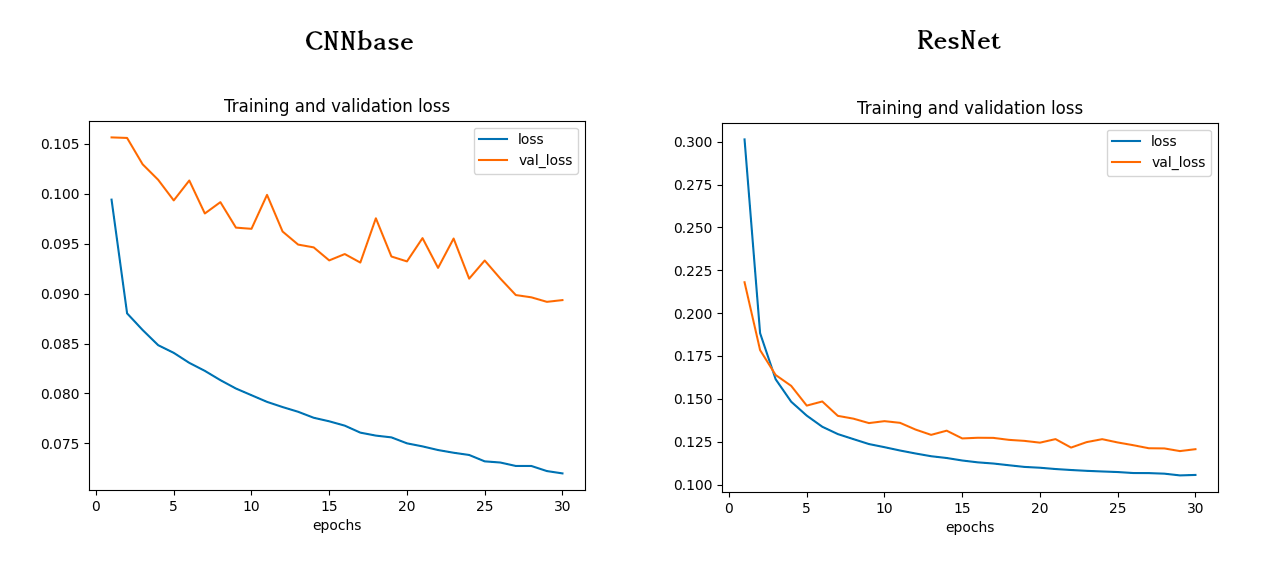
\includegraphics[scale=0.4]{Loss_accuracy_comparison_REDs.png} 
\caption{Loss Accuracy Comparison between different networks on REDs}
\label{Loss_accuracy_comparison_REDs}
\end{figure}

\section{Other Deblurring Strategies}
In this section we aim to present two further strategies to handle the deblurring problem. We tried to exlpore deep learning methods which are not attributable to the structure of autoencoders. The results are still far from being acceptable and the work would require a more in-depth research in directions that are outlined in the continuation of this section.

\subsection{Kernel Motion Estimation}
The first alternative strategy to autoencoder is a Convolutional Neural Network developed to estimate the non-uniform motion field which causes the blurring effect on each image. We applied this technique to REDs dataset because it is made up of large images (320x180) on which local intervention can be significant to handle the problem. The idea is inspired to an article by Sun et al. \cite{S&Al} and we have focused on the part of interest from a deep learning point of view. 

Our main goal is to predict the probabilities of different motion kernels for each image patch. This is the first of three phases to handle the deblurring problem and it is the only one addressed through a neural network. The second phase would be a global motion kernel prediction for the whole image, obtained by a composition of the patches kernel towards a matheamtical procedure which guarantees the smoothness property to the motion field. After that, the last phase consists in applying a deconvolution technique between the blurred image and the predicted kernel. 

A general formulation for non-uniform motion blur estimation can be adressed with the following steps:

\begin{itemize}
\item Consider non-uniform blurred image $I$ and divide it into patches.
\item For each patch $\Psi_p\in I$ we consider a motion vector $m_p = (l_p , o_p )$, which characterizes the length and orientation of the motion field.
\item Each motion vector determined a local motion kernel with non-
zero values only along the motion trace, as shown in figure \ref{motion_kernel}(a).
\item The blurry patch can be represented by $I = k(M)*I_0$ , where $I$ is the blurred image expressed as the convolution of a latent sharp image $I_0$ with the non-uniform motion blur kernels $k(M)$ determined by the motion field $M = \lbrace m_p\rbrace _{\Psi_p\in I}$.
\end{itemize}

\begin{figure}[hptb]
\centering
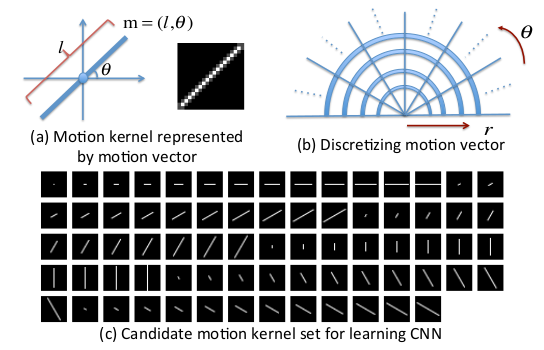
\includegraphics[scale=0.5]{motion_kernel.png} 
\caption{Representation of motion blur kernel by motion vector
and generation of motion kernel candidates}
\label{motion_kernel}
\end{figure}

We decompose our images in 20x20 non-overlapping patches and we aim to predict the probabilistic distribution of motion kernels: 
\begin{equation}
P(m = (l, o)|\Psi_p)
\label{distribution}
\end{equation}

The most interesting part for our project consists in designing a CNN as a multi-classifier, able to predict the most probable motion kernel for each patch. In the next paragraph we better discuss the architecture and a strategy to refine motion kernel estimation by considering a greater number of orientations. 

\subsection{Kernel Motion Estimation via Deep Learning}

Taking the problem of motion kernel estimation as a learning problem, we utilize convolutional neural network to learn the effective features for predicting motion distributions in equation [\ref{distribution}].

Following the approach in \cite{S&Al}, we generate a set of candidate motion kernels by discretizing the motion space. In particular, we considered 55 motion kernels as possible candidates for each patch, which are obtained considering all the possible combinations $(l,o)$ of lengths and orientations. For the discretization, $l$ assumes integer values in $[1,20]$ with step 2 (i.e. 10 possibilities) and $o$ varies in $[0^o, 180^o)$ with step $30^o$ (i.e. 6 possibilities). Note that when
the motion length l = 1, all motion vectors correspond to
the same blur kernel (identity kernel) on image grid regardless of the motion orientation, so the total number of candidates is obtained with the formula $10*6-5$. 

The architecture of the CNN has the following structure:

\begin{equation}
C1_{96}^{7,1} - M2^{2,2} - C3_{256}^{5,1} - M4^{2,2} - F5 - Dn6_{1024} - Dn7_{55}
\end{equation}

where we use the same notations introduced in section 2: $M$ stands for a Maxpooling Layer and $F$ is a flatten layer necessary for the following dense layers indicated with the label $Dn$. As activation function we always use ReLU except for the last layer, in which the multi-classification is done by using \textit{Softmax}.

Our learned CNN model can predict the probabilities of 55 candidate motion kernels in S. Obviously, this set of candidates is far from dense in the continuous motion space, therefore an extension of candiates has been introduced based on the following observation. Given a patch $\Psi_p$ we can consider 5 counterclockwise rotations of angle $\Theta \in [0^o, 30^o)$ with step $6^o$ and for each rotated patch $R_{-\Theta}(\Psi_p)$ we can use the CNN to estimate the probability distribution in \ref{distribution}. We can observe that 

\begin{equation}
P(m = (l, o+\Theta)|\Psi_p) = P(m=(l,o)|R_{-\Theta}\Psi_p) 
\end{equation}

We can therefore predict the motion distribution in an extended mo-
otion kernel set of CNN: $P(m = (l, o)|\Psi_p), o \in \lbrace 0, 6, 12, ..., 174 \rbrace, l \in \lbrace 1, 3, ..., 19 \rbrace$.
After motion kernels extension, we can totally predict probabilities of 271 candidate motion kernels for an image patch by CNN. Note that this process does not require the CNN retraining, but just feed this image and its rotated versions to our learned CNN.

After training the network with the built datset of patches on which motion blur was artificially applied, we tried to evaluate the quality of the output on a similarly constructed test dataset. The results are not satisfactory with a crossentropy index that maintains values greater than 1 even on the training dataset. On one hand, the network seems to learn during the first 6 epochs with a significant decrease in the crossentropy value; after the 15th epoch the crossentropy on the training dataset still seems to be in a considerable decrease trend. On the other hand, the validation set begins to ease the decrease already from the 6th epoch and shortly thereafter it starts to grow again showing a typical overfitting behavior (figure \ref{motion_kernel_SSIM}).

\begin{figure}[hptb]
\centering
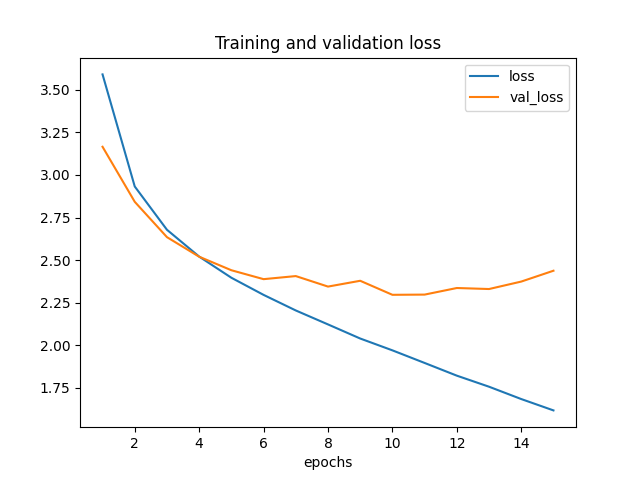
\includegraphics[scale=0.45]{KernelMotion_loss.png} 
\caption{SSIMLoss value for Kernel Motion Estimation}
\label{motion_kernel_SSIM}
\end{figure}

Considering the promising results shown in \cite{S&Al} we think that further research could lead to better outputs for our network. For example, it might be worthwhile to extend the training dataset by increasing the number of patches considered. To date we have worked with 82500 "artificial blurred" patches, extracted from 3 frames in 100 videos of the REDS traning dataset. For each frame we have randomly chosen 5 patches and applyed the 55 motion vectors mentioned above. Maybe there is not enough variety in the built dataset and it could be increased by considering more videos from which to extract the frames. 

\subsection{Style Transfer}
As regard the second technique, we tried to investigate another approach, based on the neural style transfer \cite{G&E&B} \cite{Site}. In the following, it is explained how this technique works and then how we used it to try to solve the deblurring problem for the CIFAR10 dataset.

Neural style transfer is an optimization technique used to take two images, a content image and a style reference image, and blend them together so the output image looks like the content image, but “painted” in the style of the style reference image.
This is implemented by optimizing the output image to match the content statistics of the content image and the style statistics of the style reference image. These statistics are extracted from the images using a convolutional network.

In practice, a pretrained image classification network called VGG19 was used. Some internal convolutional layers of this model have been extracted, in order to define the representation of content and style from the images. This requires taking the raw image as input pixels and building an internal representation that converts the raw image pixels into a complex understanding of the features present within the image. Thus, somewhere between where the raw image is fed into the model and the output classification label, the model serves as a complex feature extractor. By accessing intermediate layers of the model, we are able to describe the content and style of input images.

The content of an image is represented by the values of the intermediate feature maps. It turns out that the style of an image can be described by the means and correlations across the different feature maps. Calculating the gram matrix for a particular layer gets these informations.
After defining an extractor model, which returns the style and content tensors, we can now implement the style transfer algorithm. This is done calculating the mean square error for the image's output relative to each target, then taking the weighted sum of these losses. More in depth, at each iteration the custom loss function computes the distance between the style of the content image and the style image and the distance between the respective content features. The first matters very little, because the content image has to preserve its main features. The latter matters a lot, for the same previous reasons. At each iteration the otpimizer tries to bring the image closer to the style, according to the loss function.

Our approach is based on this technique. We hypothesised the deblurring problem as a particular style transfer problem. In fact, we thought about the content image as the blurred image, which has to learn the sharp style. To do that, without having the sharp image, we decided to show not only a single style image, but an entire dataset. These style images had completely different shapes and colours, but they had something in common: the sharpness. So, we tried to adjust the weight parameters in order to teach the content image for just a little information, which contains the colours and the shape of the style image, but also the sharpness of it. We supposed that for high numbers of images, the randomness of the first two features would have disappeared, allowing the common feature of the sharpness to spread all over the blurred content image.
\begin{figure}[hptb]
\centering
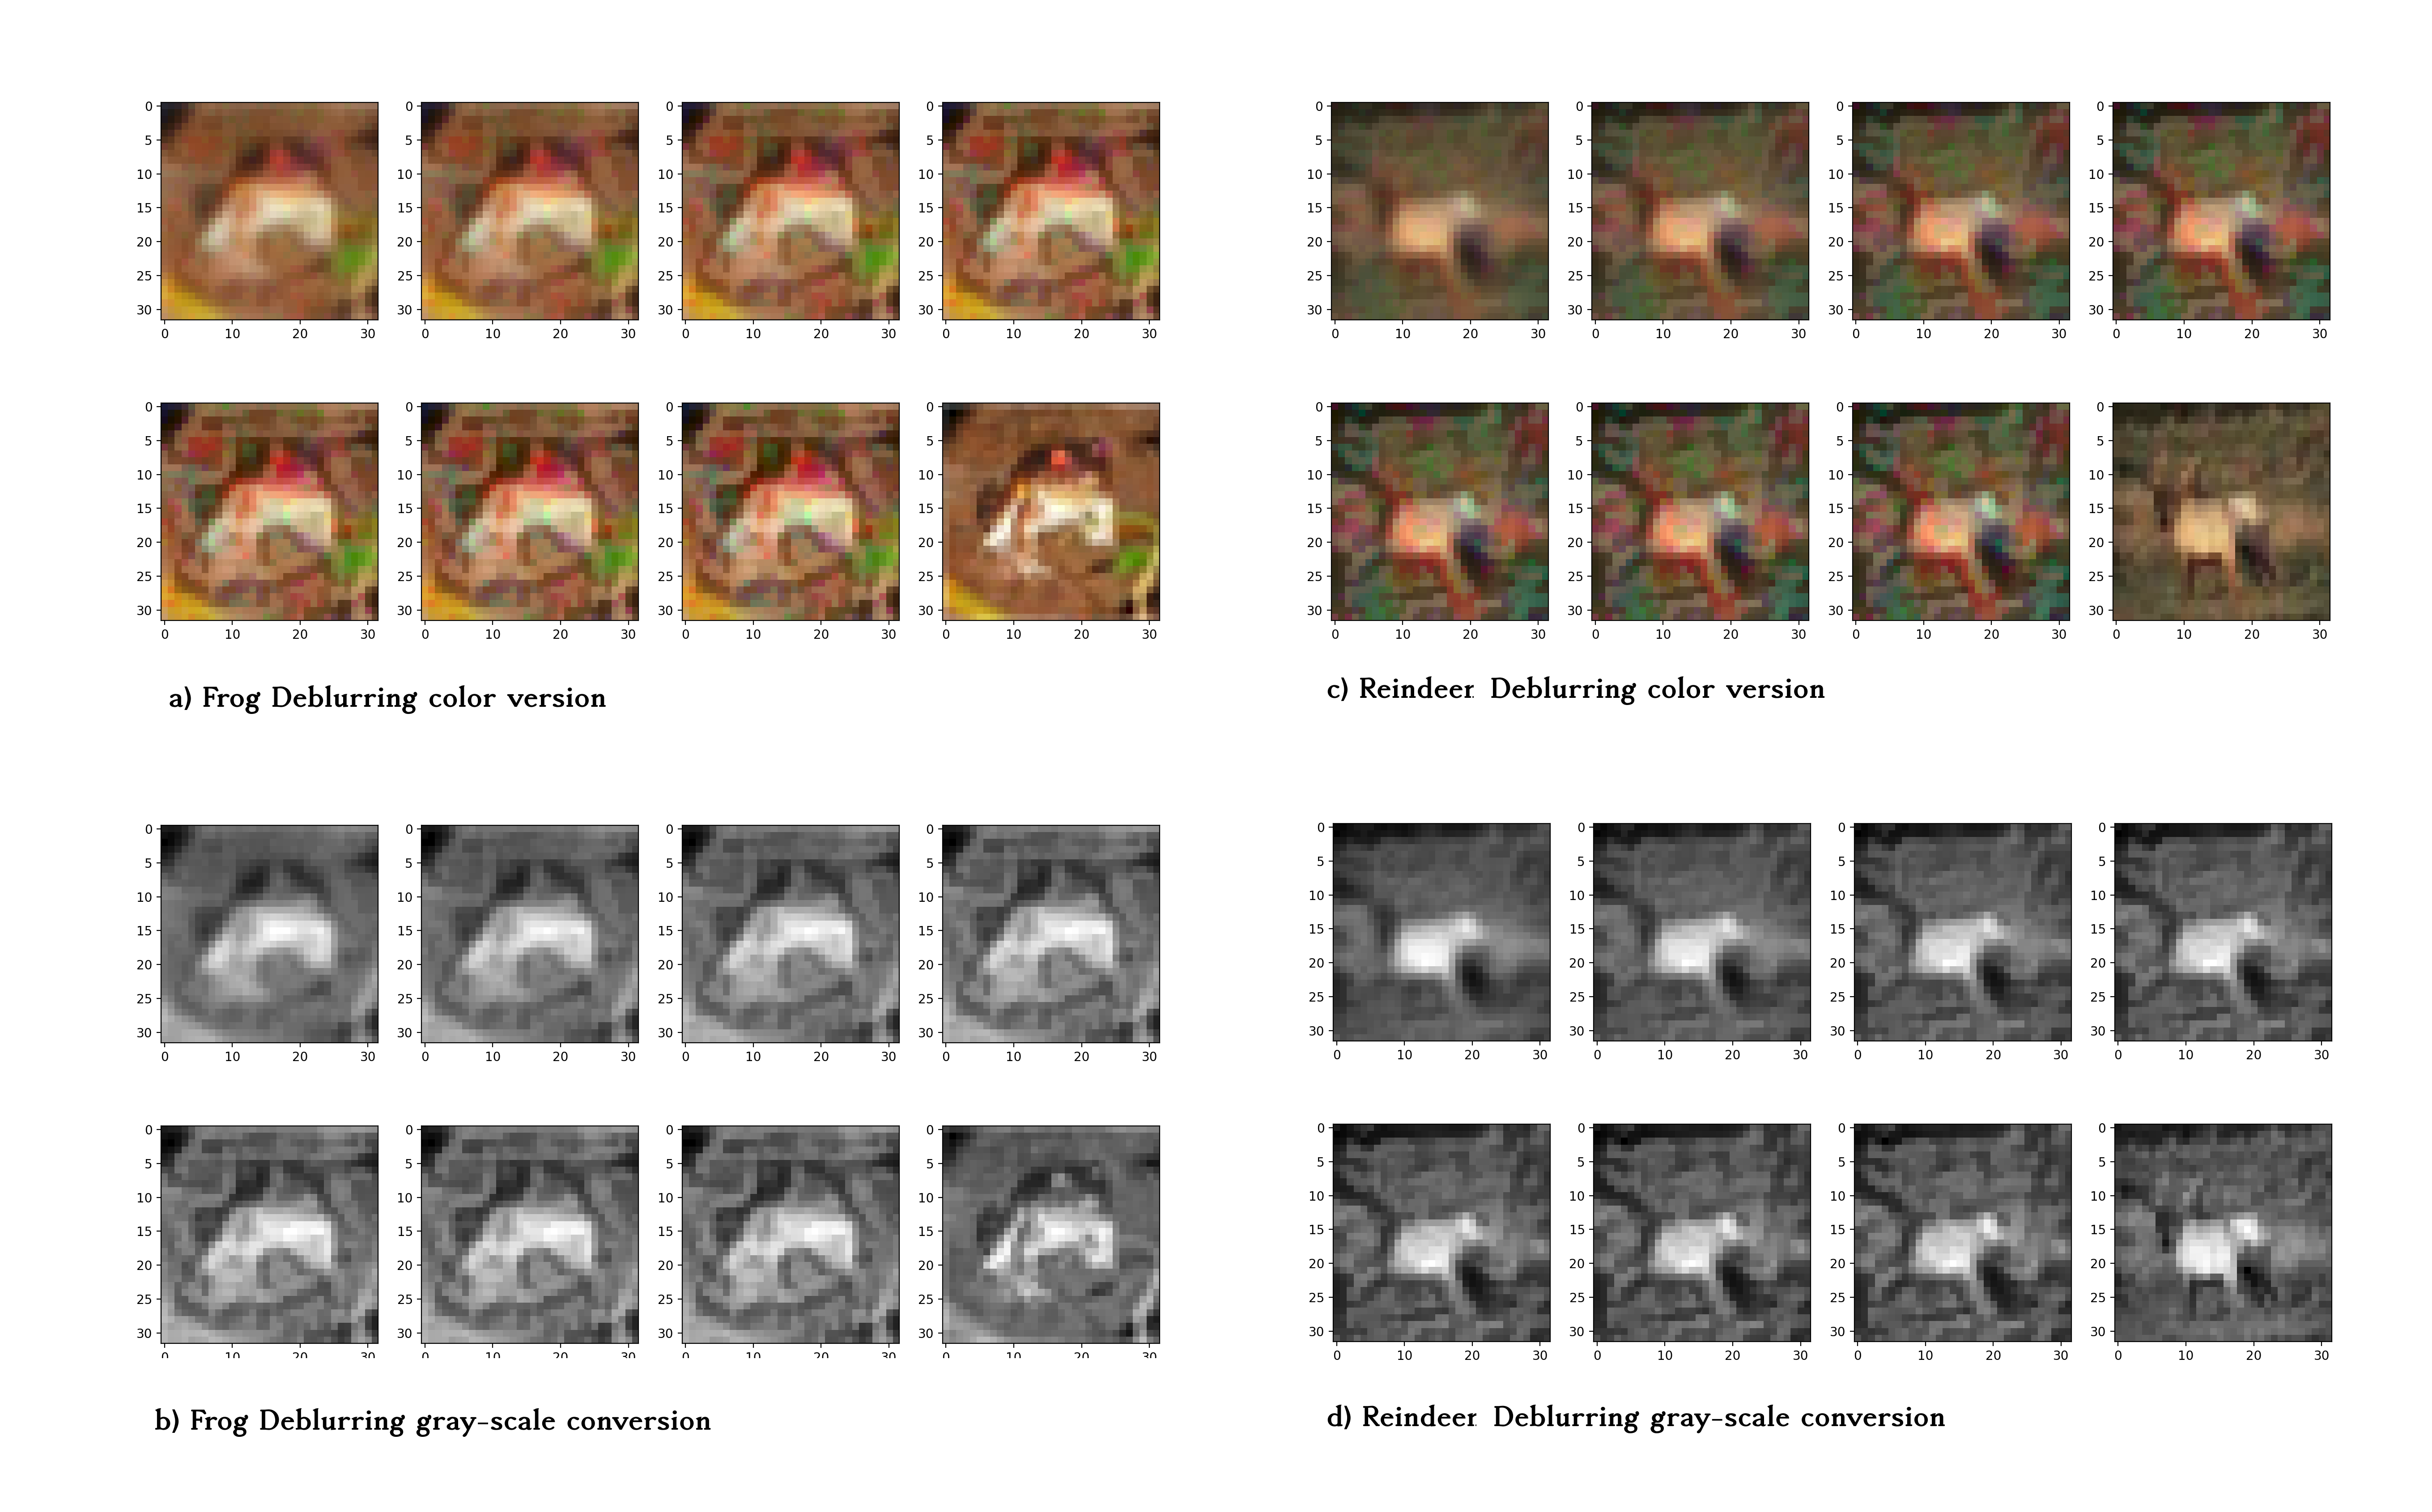
\includegraphics[scale=0.1]{style_outputs.png} 
\caption{Style Transfer outputs on two images of CIFAR10. The last image in each group is the sharp image.}
\label{style_outputs}
\end{figure}

Unfortunately, the results are not so good. As we can see from the results in figure \ref{style_outputs}, the image gradually acquires sharpness, even if it does not recover the original shapes of the image and there is a color problem in the restored image. It could be interesting to see if with a dataset of black and white images the results obtained are better because they are not influenced by the chromatic range of the different images. In addition, the search could be deepened by choosing differently the output layers used to define the style, trying to identify those that best intercept the desired texture. We limited ourselves to a final black and white conversion of the output images only to visually assess whether the quality improved. 

\begin{figure}[hptb]
\centering
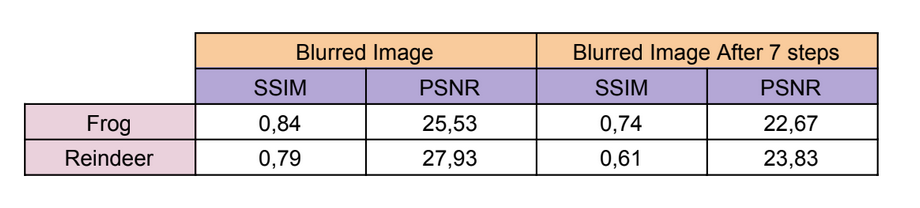
\includegraphics[scale=0.5]{style_transfer.png} 
\caption{Crossentropy values for Style Transfer}
\label{style}
\end{figure}

Also the PSNR and SSIM metrics confirm the poor quality of the results as shown in the table in  figure \ref{style}. However, it is interesting for us to report an attempt that has not yet been investigated in the literature.

\section*{Conclusion}
\addcontentsline{toc}{section}{Conclusion}
In the project we have widely explore different autoencoder strategies and we have also tried to investigate two different approaches. The autoencoder in its plain version seems to produce the best results on both dataset and we did not really appreciate the advantages of Skip Connections and ResNet mentioned in the literature such as, respectively, the faster decrease of the loss function and the reconstruction of the shapes of the objects in the images. However the Skip Connection networks recover the original colors better than the similar CNN Base networks and this is particularly visible in some images of the CIFAR10 sample.

As regard a comparison of different structure of the same architecture, we can state that the shallower networks have better results. Moreover, the use of an higher number of filters seems to have a positive effect on the accuracy in color recovery.

As for the metrics, the use of SSIM in the definition of the loss function is more adequate than MSE and, in accordance with the suggestions in the literature, we have given priority to maximizing SSIM over PSNR.

The other two presented strategies did not produce the desired results and perhaps this explains why even the literature contains fewer references to them. However, the possibility of exploring these paths remains open as already discussed in the dedicated paragraph.


A possible development strategy about autoencoder networks would be to try to further modify the CNNBase networks in the first version, by increasing the number of filters at the expense of a slightly larger stride.

\newpage

\newpage
\begin{thebibliography}{99}
\bibitem{P&V&G}  Patel, Amit and Vankawala, Fagun and Ganatra, Amit. (2015). A Survey on Different Image Deblurring Techniques. International Journal of Computer Applications. 116. 10.5120/20396-2697. 
\bibitem{H&Al} I.M. El-Henway et Al. (2014). A comparative study on Image Deblurring Techniques. International Journal of Advances in Computer Science and Technology. Vol 3. No 12.
\bibitem{M&Al} Mao, Xiao-Jiao and Shen, Chunhua and Yang, Yu-Bin. (2016). Image Restoration Using Convolutional Auto-encoders with Symmetric Skip Connections. 
\bibitem{N&Al} Nimisha, T and Kumar Singh, Akash and Rajagopalan, A. (2017). Blur-Invariant Deep Learning for Blind-Deblurring. 4762-4770. 10.1109/ICCV.2017.509. 
\bibitem{H&X&R} He, Kaiming and Zhang, Xiangyu and Ren, Shaoqing and Sun, Jian. (2016). Deep Residual Learning for Image Recognition. 770-778. 10.1109/CVPR.2016.90. 
\bibitem{Z&G&F} Zhao, Hang and Gallo, Orazio and Frosio, Iuri and Kautz, Jan. (2016). Loss Functions for Image Restoration With Neural Networks. IEEE Transactions on Computational Imaging. PP. 1-1. 10.1109/TCI.2016.2644865.
\bibitem{W&B} Wang, Zhou and Bovik, Alan and Sheikh, Hamid and Simoncelli, Eero. (2004). Image Quality Assessment: From Error Visibility to Structural Similarity. Image Processing, IEEE Transactions on. 13. 600 - 612. 10.1109/TIP.2003.819861. 
\bibitem{G&E&B} L. A. Gatys, A. S. Ecker and M. Bethge, "Image Style Transfer Using Convolutional Neural Networks," 2016 IEEE Conference on Computer Vision and Pattern Recognition (CVPR), Las Vegas, NV, 2016, pp. 2414-2423, doi: 10.1109/CVPR.2016.265.
\bibitem{S&Al} J. Sun, Wenfei Cao, Zongben Xu and J. Ponce, "Learning a convolutional neural network for non-uniform motion blur removal," 2015 IEEE Conference on Computer Vision and Pattern Recognition (CVPR), Boston, MA, 2015, pp. 769-777, doi: 10.1109/CVPR.2015.7298677.
\bibitem{Site} \url{https://www.tensorflow.org/tutorials/generative/style_transfer}

\end{thebibliography}

\end{document}